\begin{figure}[h!]
	\centering
 	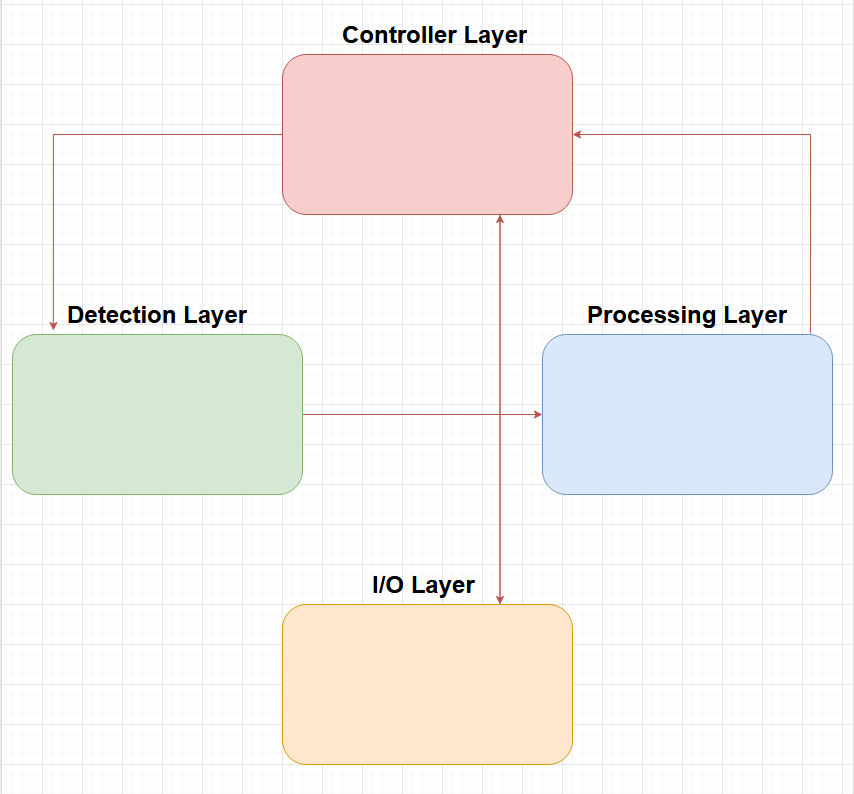
\includegraphics[width=1\textwidth]{images/adslayoutclean.png}
 \caption{A simple architectural layer diagram}
\end{figure}

\subsection{Layer Controller Description}
The controller layer's main purpose is to control and regulate the entirety of the system.  The main interface is the raspberry pi; it communicates to sensors in the detection layer on when to activate, as well as takes information from the processing layer and sends that information to the drone database subsystem.  Additionally, the raspberry pi takes input from users and adjusts settings on the system.

\subsection{Layer Detection Description}
The detection layer consists of sensor subsystems:  acoustic arrays and a secondary detector.  These sensors take in real-world-analog data and transfers that data over to the processing layer to be digitized and processed further.  Also, the secondary detector subsystem is pinged by the controller layer.

\subsection{Layer Processing Description}
Within the processing layer, the analog to digital converter (ADC) is the internal interface, of which it digitizes analog data and sends it to the ODAS subsystem as well as the secondary processor subsystem.  Finally, the processed data from the ODAS and secondary subsystems are sent to the controller layer, into the raspberry pi subsystem.

\subsection{Layer I/O Description}
The Input/Output layer's main purpose is to provide the interface to the user to graphically view the detected drones and select individual detected drones to track actively. The layer communicates both ways with the controller layer to receive the data of the detected drones and display it and also send the input from the user.